\newpage
\section{Questions and Answers} \label{answers}

% This section can be added when the tutorial is finished, so the students can check if their answers are correct.

This section will guide you or give answers to the questions asked during the tutorial. First, the question is repeated, and after \cmd{-} or \cmd{:}  there will be an answer. The questions are numbered the same as the ones in the text earlier.

%\subsection*{Preparation}

\begin{enumerate}
    \item How do you think making notes during the tutorial will benefit you? - No answer given. Personal statement from the student. The student gives a short statement of why taking notes is beneficial (or not) when doing a tutorial.
    \item What is a hash? - A hash is a value that is calculated from the file. It is used to verify data authenticity. If a hash is calculated on a file, it will never change unless the file is changed.
    \item Did your hash values match?: - If the values do not match, check if you did it correctly.
    \begin{itemize}
        \item In Windows: Start and CMD or PowerShell prompt and use the command: \cmd{certutil -hashfile <NAME OF YOUR FILE> SHA256}
        \item In Ubuntu: Start your terminal and use the following command: \cmd{sha256sum <NAME OF YOUR FILE>}
    \end{itemize}
    \item Why do you create a virtual network? - If this were a physical lab, you would have used switches, cables, and other network devices to create a physical network, to make the clients talk to each other. When it is done virtualized, you need the same, but the virtual network is emulating those physical devices in your network. Another reason is that you are now segregating the network from your original host network.
    \item What does the \cmd{em} in the network card stand for? - em references to the manufacturer of the network adapter. em = intel and for example bge = Broadcom.
    \item Why did you remove the checkmark for RFC1918 Networks? - Since the IP's you are using are private IP's you need to remove the checkmark. If you do not remove it, IP's that are private cannot be used. \url{https://tools.ietf.org/html/rfc1918}.
    \item Can you ping your firewall from your client? - Use the ping command. \cmd{ping 192.168.20.1}. On Linux, use \cmd{CTRL + C} to stop the ping command or use the \cmd(-c 3) to limit the amount of ping sent to three (3).
    \item What is key-size? - Key-size is the length of bits that are used by the algorithm when generating cryptographic keys.
    \item What is the difference between a private key and a public key? - Private key is your key and must be kept secret. The public key is the key that can be shared and given to for example a server that you want to login to.
    \item What does the \cmd{Password protect the console menu} checkbox in \cmd{System -> Settings -> Administration} in the web GUI do? - It makes it impossible to change the password, without having physical access to the firewall.
    \item Try to ping your client. Do you get something similar to figure \ref{opensense:admin_ping}? - Answered in the section. See figure \ref{opensense:admin_ping}.
    \item Why do you think the action \cmd{Reject} is mostly used on so-called friendly networks? - To save time for the client that is trying to connect, it is important that the client knows that the request is blocked. This can save time for troubleshooting.
    \item Try now to \cmd{PING} the same website as you did in bullet point 4. What is happening? - If it is done correctly, you are not able to ping any websites.
    \item How can you disable the rule that was created? - By clicking on the red cross in the overview of the firewall rules.
    \item Are you able to ping any website from the Ubuntu Server when the rule is disabled? - Yes.
    \item Do you see any evidence in the log when the rule that was created earlier is active? - It should be possible to see something like figure \ref{opnsense:logging_blocked_internet_access} in the log.
    \item How can you test if this is working? - See \ref{python_server}
    \item Play around and try to create other rules. - The student can try to allow FTP or Telnet and test if it is working.
    \item Where in the rule editor page can you add the time-based rule? - When the time-based rules are created, it is possible to choose it under the \cmd{Schedule} options almost at the bottom of the rule edit page.
    \item Try to create a schedule and add it to a rule that blocks access to \cmd{www.nrk.no} inside the normal working hours (08.00 - 16.00). - 
    \item Can you create a firewall rule that uses the alias you created to block one country? -
    \item How can you test if the previous create rule is working? -
    \item Is it possible to do a packet capture with \opnsense? - Yes it is possible. Goto \cmd{Interfaces --> Diagnostics --> Live View --> Packet Capture}.
    \item What is outbound NAT? - Easy explained; it translates the internal IP in packets to the WAN IP on outgoing packets, and reverse on incoming packets.
    \item Is it working? - Try to browse the internet.
    \item What does port forward do? - Expose a service that is run on an internal IP address to a port on the WAN side of your network.
    \item What can be done to improve the security when port forwarding is used? - Set up firewall rules, use HTTPS instead of HTTP and general hardening for the service and the server.
    \item Why would you put the management of the firewall and other network devices on a separate network? - When it is on its own network, it will not slow down or fail during periods with high load on the firewall.
    \item Test the configuration you have made, using a site that can do speed tests. Do you get the same result as in figure \ref{opnsense:bandwidth_speed}? - Answer is given in the question.
    \item How can you use this rule against on IP instead of all on the interface? - Change the Source and Destination in the \cmd{Firewall --> Shaper --> Rule} to the IP you want to limit.
    \item There is also one more configuration that can be done, \cmd{queues}. What does it do? - It can be used to creates flow (one or multiple) in a pipe. It can prioritize which flow in a pipe is getting access to the bandwidth first or need to wait. Can also choose how the bandwidth in the pipe is divided by source or destination. Mainly pipes are used to hard limits and queues to give hosts a different share of the flow in a pipe.
    \item Why would you prioritize some traffic over other traffic? - A good example could be the IP telephone. You would prioritize the IP telephone over for example a user that is streaming something or downloading something. This will be useful especially if there are a lot of users or the ISP cannot deliver a fast line.
    \item How can you test if the queue is working? - Create a pipe. Then create 2 queues. It is important that they are weighted differently. Then create one rule for each of the queues that were created. When the rules are created, use different protocols. For example FTP, HTTP or something else. To test this, start something that creates traffic for the protocol that has the highest weight first, and see what happens when you starts to create traffic on the other protocol. A good idea is to use for example HTTP/HTTPS on the rule with the high weight (easy to start a download to saturate the pipe.).
    \item Find the \opnsense\ WAN IP address and try to access it from your host. Does it work? - Find the WAN IP address on the \cmd{Lobby --> Dashboard} page on your firewall, and insert https:// before the WAN IP when trying from the host machine.
    \item Did you manage to connect to the firewall? - If you managed to connect, you will see it in the \cmd{VPN --> OpenVPN --> Connection Status} page.
    \item What is the minimum recommended key size for RSA encryption? - NIST (National Institute of Standards and Technology) recommends at least 2048 bits (\cite{Barker}). This recommendation can be different in other organisations and will be higher when years go by.
    \item What are regular expressions? - Regular expressions are used to match patterns in a string.
    \item What is the difference between using \cmd{nrk.no} and \cmd{https://www.nrk.no} when filtering? - The difference is that it filters on the exact string that is used. So \cmd{nrk.no} will be found everywhere in the URL, versus \cmd{https://www.nrk.no} will be only found first in a URL. 
    \item How can you use a whitelist instead of a blacklist? - Insert a \cmd{.} in the blacklist and start using the whitelist.
    \item Use some time and see if you can find another list that can be used. - Explore the lists.
    \item How can you test if the Shallalist is working? Just explain it, do not try to do it. - WARNING: A solution can be to go to a page that is in the block list. THIS IS NOT RECOMMENDED!!
    \item How can you configure \opnsense\ to automatically update the rule list? - Use the \cmd{Schedule with Cron} button to create a scheduling task.
    \item Explorer the three logs and explain what they log. - This is a logfile from Squid. \cmd{Cache log} is the cache.log file. It stores information about configuration, warnings and errors. \cmd{Access log} is the access.log file. It is used to store client requests. And the  \cmd{Store log} is the store.log file. It stores the decisions made by Squid to store and remove objects from the cache.
    \item Try to test the IDS using a EICAR rule that has a \textbf{https} (\url{https://secure.eicar.org/eicar.com.txt})? Why do you think it is not working? - The IDS cannot see data that is in an encrypted packet, since the encryption/decryption is happening on each endpoint. If the firewall should inspect encrypted packets a proxy need to be configured.
    \item Try to add the OPNsense social media ruleset and go to one of the well known social media sites. What happens in the log? - If you goto \url{https://facebook.com} you will get multiple alerts in your log.
    \item What does DNS do? - DNS makes it easier to navigate the internet. Instead of remembering each individual IP address, you can remember a name. DNS translate Ips to human readble names.
    \item Can you explain what DHCP is? - DHCP is a service that gives Ips to each device that is connected.
    \item How could you check if routing is working? - Using the ping command, see \ref{ping} and disable packet filtering, see \ref{pk_capture}.
    \item When is it useful to use an external NetFlow collector? - When there are multiple sources of data, that is merged. For example, a company that has multiple firewalls and maybe servers that can send NetFlow data.
    \item Play around with the export function and see if you can find some opensource tool and import the data too. - A cool open-source tool is https://github.com/robcowart/elastiflow.
\end{enumerate}

\begin{figure}[h!]
    \centering
    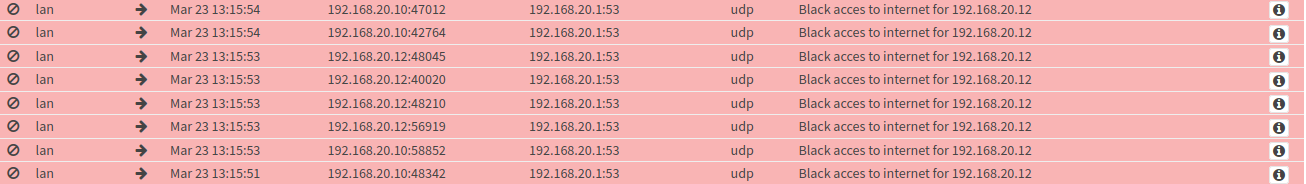
\includegraphics[width=0.9\textwidth]{Images/firewall/block_internet_access.PNG}
    \caption{\opnsense\ logging of rule that blocks all internett access}
    \label{opnsense:logging_blocked_internet_access}
\end{figure}

